\label{chapter:applications}

To demonstrate the impact of GATs, we will present two examples for their applications. The first one was developed in collaboration with some of the involved authors shortly after the original paper was published. Then, a fairly recent publication will highlight the relevance of the architecture to this day.

\section*{GATs for Brain Mesh Segmentation}
In \cite{Cucurull2018ConvolutionalNN}, both GCNs and GATs were cutting edge technologies that were assessed against previous mesh parcellation models. Reconstructions of the cortical surface were represented in a graph which had to be divided into areas. Nodes correspond to locations on the brain surface, their features included cortical thickness, curvature and functional connectivity. \\

The authors considered three kinds of information that the models could use: \textit{neighborhood information}, \textit{node features} and \textit{global information}, that is, access to feature information from all the nodes. 
Previous approaches for this task were unable to exploit all three kinds of information and were therefor limited in their complexity. Alongside GCNs, GATs outperformed all state-of-the-art models, showing the importance of utilizing the mesh structure in the data. Furthermore, the authors showed that dynamic attention mechanisms actually improve performance when compared to a constant attention for all neighbors.

\begin{figure}[h]
    \centering
    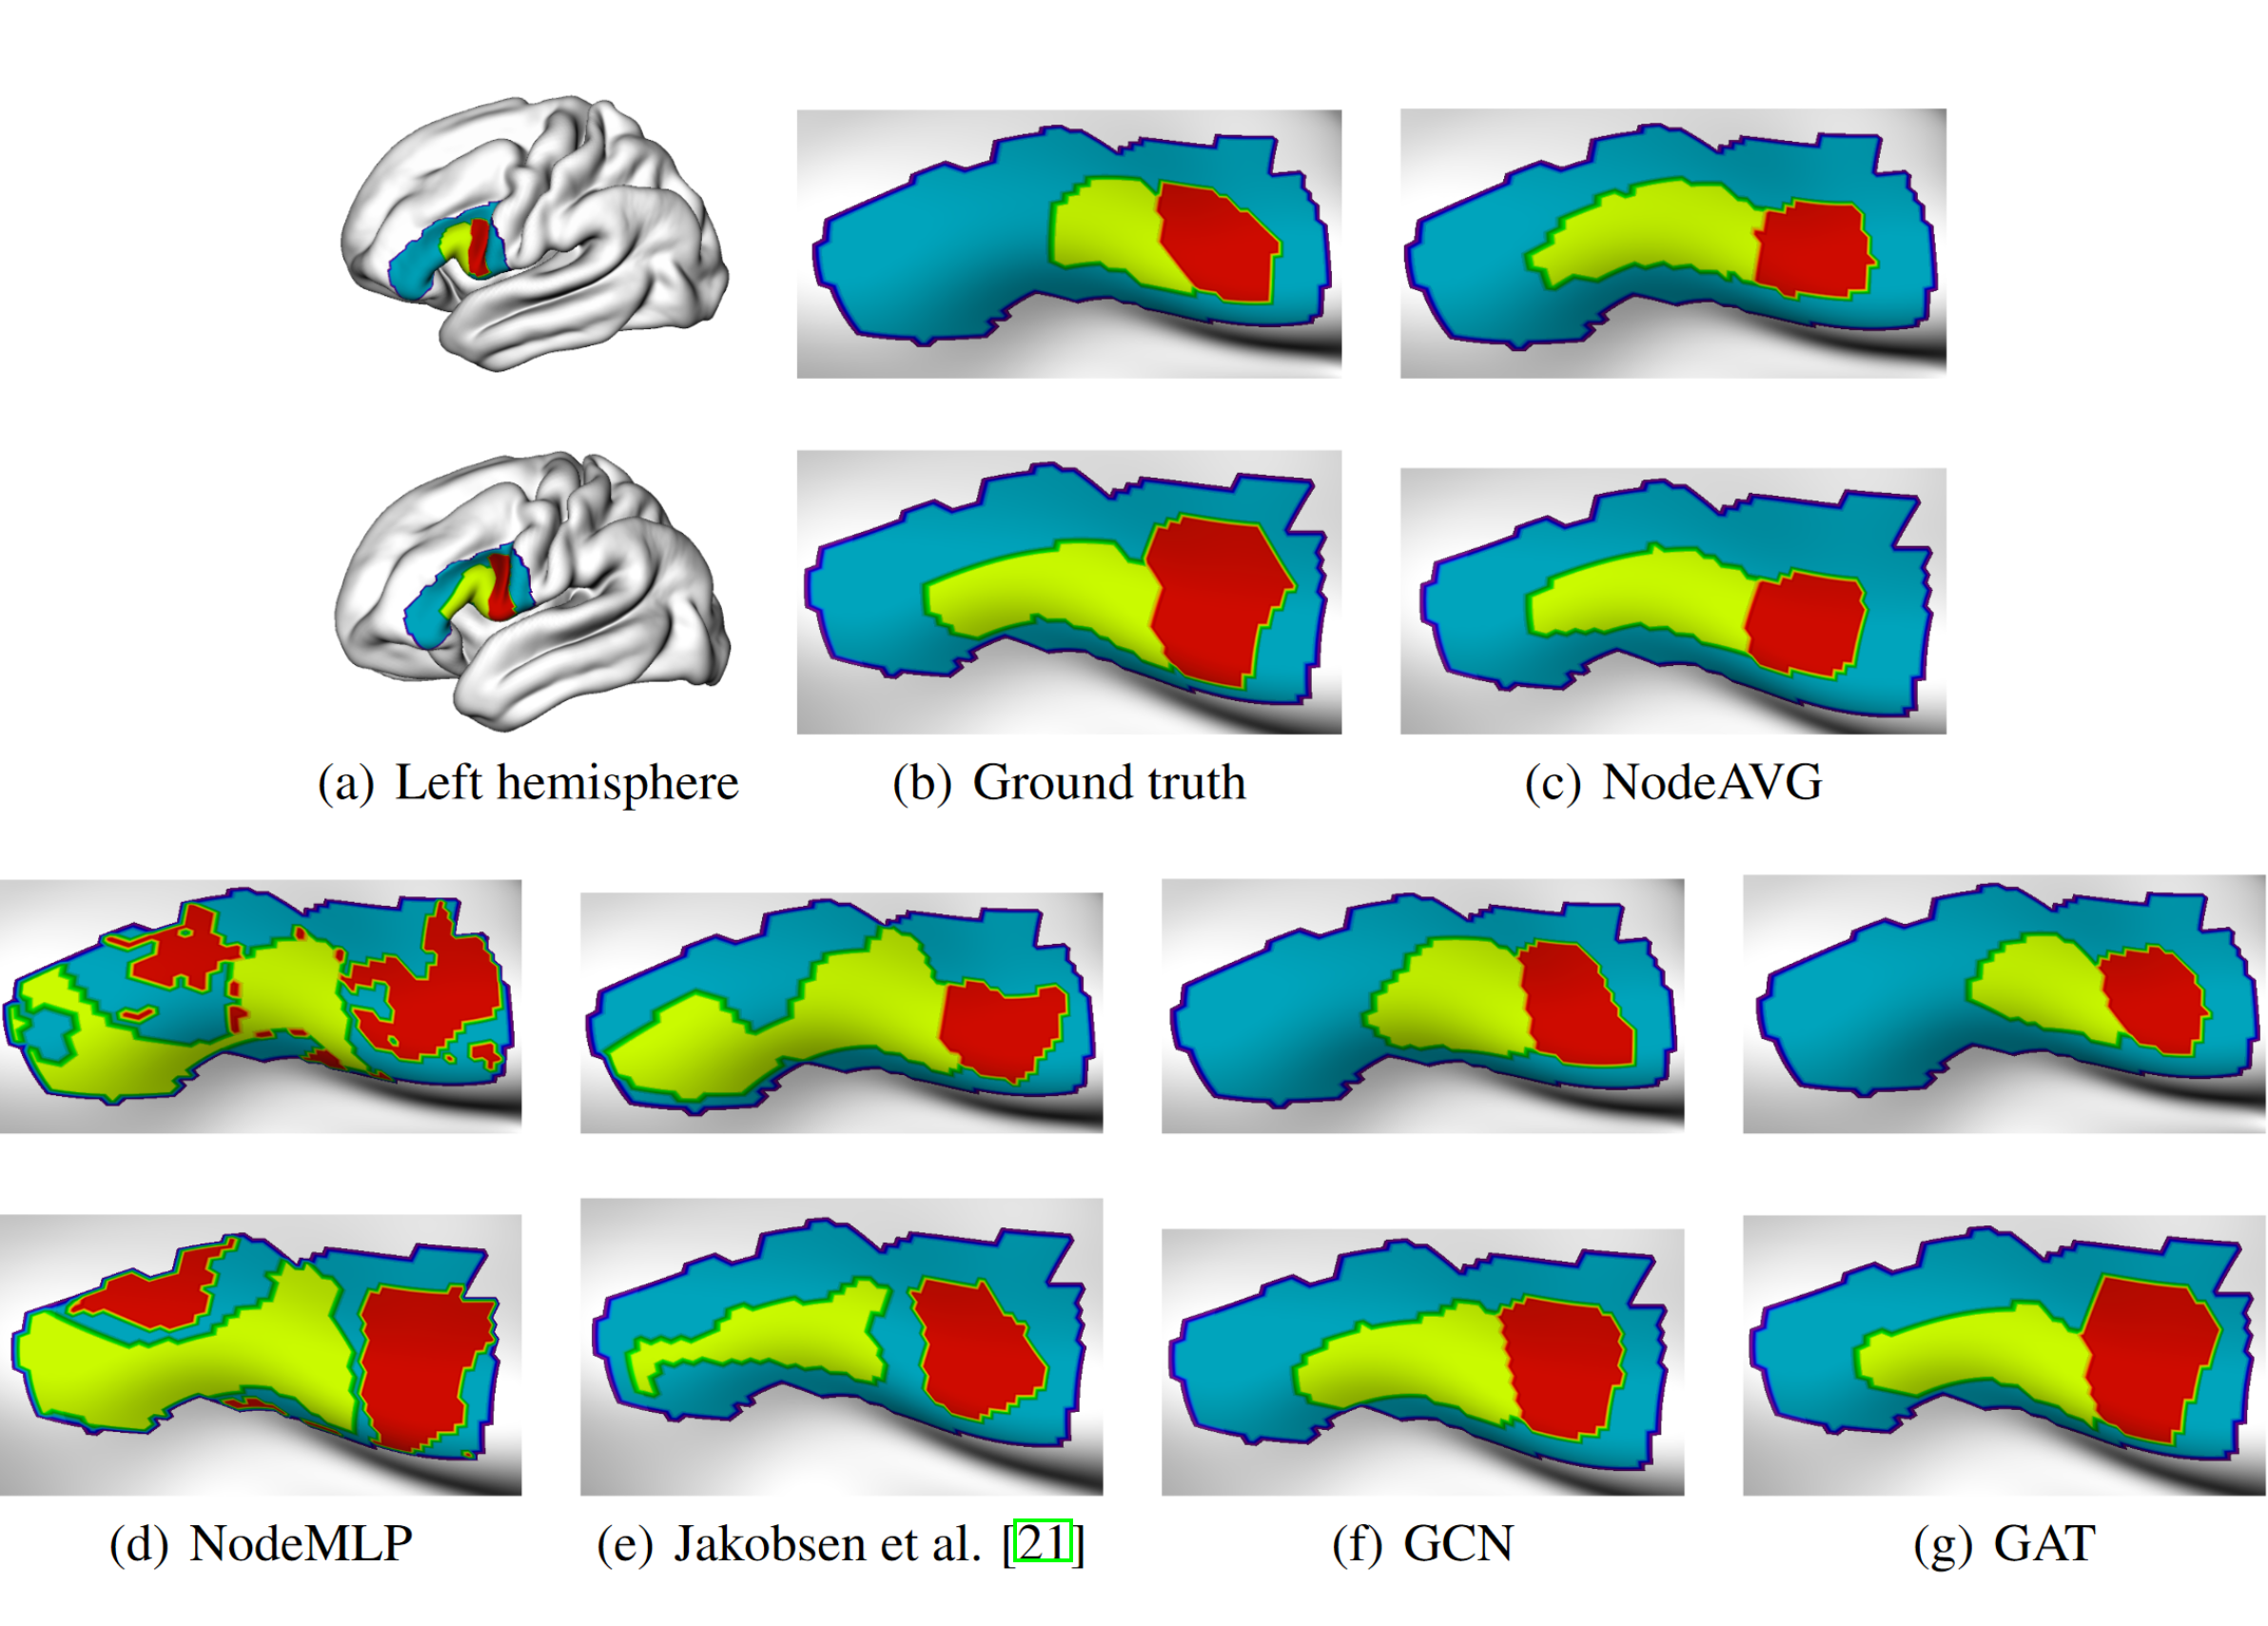
\includegraphics[width=0.75\textwidth]{img/brain_mesh.PNG}
    \caption{Qualitative area parcellation results for two test set subjects. \cite{Cucurull2018ConvolutionalNN}}
\end{figure}

In conclusion, this application demonstrated the potential of GNNs and their applicability to real-world problems. GATs showed promising results, raising hopes for applications in other areas. As we will see later on, this assessment is still up to date and in-line with recent benchmarks.\\~\\
